\documentclass[convert={density=600,outext=.png}]{standalone}
\usepackage{tikz, pgfplots}
\usepackage{xcolor}

\renewcommand{\familydefault}{\sfdefault}

\usepackage{sansmath} % sans serif math                                                                                                                               
\sansmath % if you use it globaly                                                                                                                           

\usetikzlibrary{shapes, arrows, fit, backgrounds, positioning}

\begin{document}
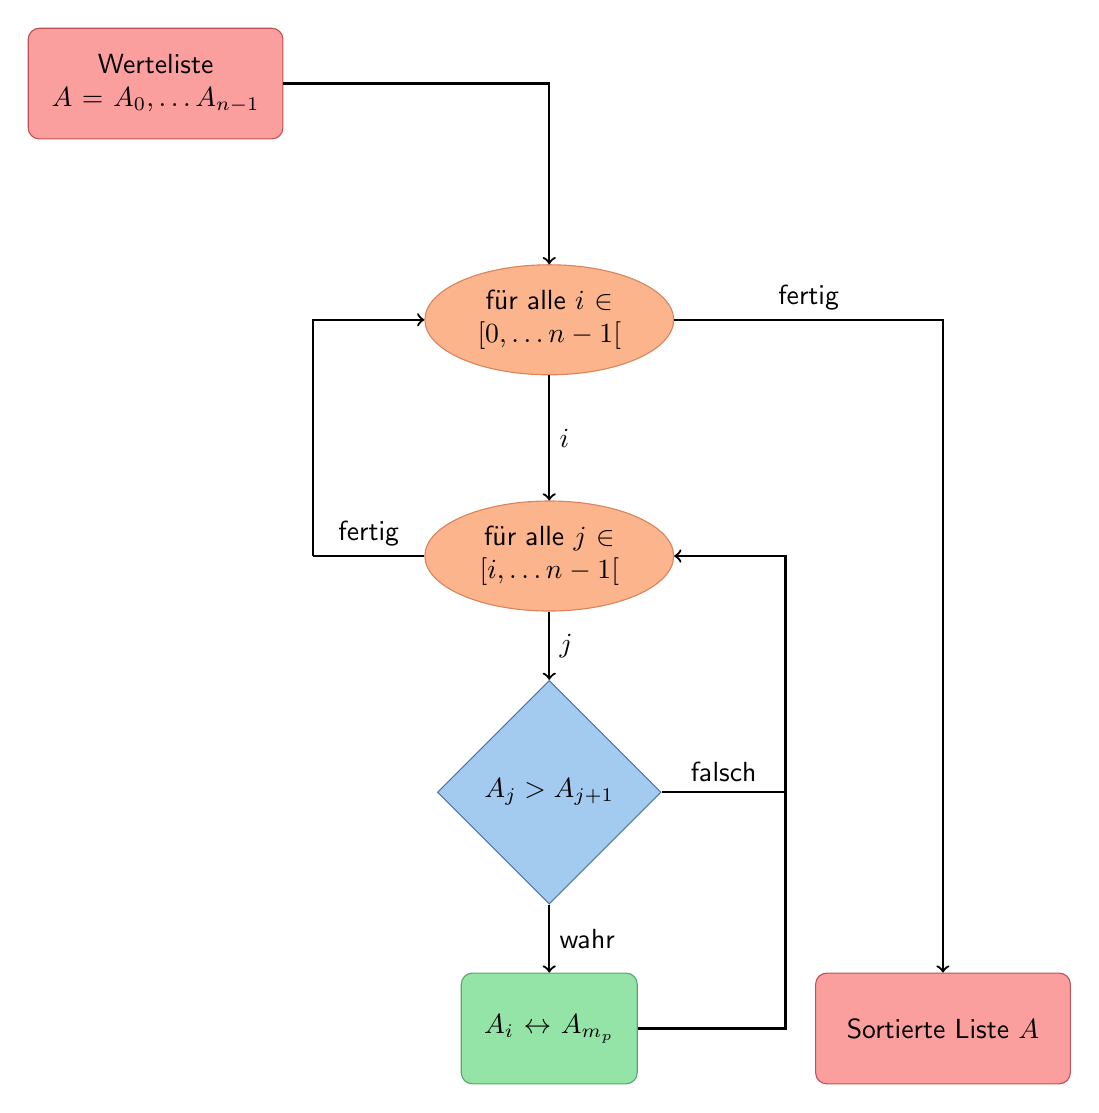
\begin{tikzpicture}[node distance=3cm and 5cm, on grid]

	\definecolor{my_blue}{RGB}{80,116,172}
\definecolor{my_blue_light}{RGB}{163,203,240}

\definecolor{my_orange}{RGB}{217,132,92}
\definecolor{my_orange_light}{RGB}{251,180,139}

\definecolor{my_green}{RGB}{91,166,108}
\definecolor{my_green_light}{RGB}{148,228,167}

\definecolor{my_red}{RGB}{192,80,86}
\definecolor{my_red_light}{RGB}{251,159,158}	

\definecolor{my_gray_dark}{RGB}{60,60,60}

\tikzstyle{decision} = [diamond, draw, draw=my_blue, fill=my_blue_light, text width=2.5cm, text badly centered, inner sep=0pt]
\tikzstyle{block} = [rectangle, draw=my_green, fill=my_green_light, text width=2cm, text centered, rounded corners, minimum height=4em]
\tikzstyle{blockio} = [rectangle, draw=my_red, fill=my_red_light, text width=3cm, text centered, rounded corners, minimum height=4em]
\tikzstyle{cloud} = [text centered, ellipse, draw=my_orange, fill=my_orange_light, text width=2cm, minimum height=3em]
\tikzstyle{line} = [draw, thick]

\tikzstyle{back_box} = [draw=my_gray, fill=my_gray_light, behind path]

	\node [blockio] (eingabe) {Werteliste\\$A=A_0, \dots A_{n-1}$};
  
	\node [cloud, below right=of eingabe] (loop1) {für alle $i\in [0,\dots n-1[$};

	\node [cloud, below=of loop1] (loop2) {für alle $j\in [i,\dots n-1[$};

	\node [decision, below=of loop2] (check_max) {$A_j > A_{j+1}$};

	\node [block, below= of check_max, node distance=3cm] (swap) {$A_i \leftrightarrow A_{m_p}$};

	\node [blockio, right=of swap] (ausgabe) {Sortierte Liste $A$};

	\node [coordinate, left of=loop2, node distance=3cm] (c1) {};
	\node [coordinate, right of=check_max, node distance=3cm] (c2) {};
	
	
	\path [line, ->] (eingabe) -| (loop1);
	\path [line, ->] (loop1) -- node [midway, right] {$i$} (loop2);  
	\path [line, ->] (loop1) -| node [near start, above] {fertig}  (ausgabe);  

	\path [line, ->] (loop2) -- node [midway, right] {$j$} (check_max);  
	\draw [line] (loop2) -- node [midway, above] {fertig}  (c1);  
	\path [line, ->] (check_max) -- node [midway, right] {wahr} (swap);     
	\draw [line] (check_max) -- node [midway, above] {falsch} (c2);
	\draw [line] (swap) -| (c2);
	\draw [line, ->] (c2) |- (loop2);
	\draw [line, ->] (c1) |- (loop1);
%	\draw [line, ->] (swap) |- (loop1);
	

\end{tikzpicture}
\end{document}
